\documentclass[a4paper, 11pt]{article}
\usepackage[polish]{babel}
\usepackage[MeX]{polski}
\usepackage[utf8]{inputenc}
\usepackage[T1]{fontenc}
%\usepackage{times}
\usepackage{graphicx,wrapfig}
%\usepackage{anysize}
%\usepackage{tikz}
%\usetikzlibrary{calc,through,backgrounds,positioning}
\usepackage{anysize}
\usepackage{float}
%\usepackage{stmaryrd}
%\usepackage{amssymb}
%\usepackage{amsthm}
%\marginsize{3cm}{3cm}{3cm}{3cm}
%\usepackage{amsmath}
%\usepackage{color}
%\usepackage{listings}
%\usepackage{enumerate}

\author{Marcin Jędrzejczyk,Paweł Ogorzały}
\newcommand{\HRule}{\rule{\linewidth}{0.5mm}} % Defines a new command for the horizontal lines, change thickness here
\newtheorem{defi}{Definicja}
\begin{document}
	% \noindent -  w tym akapicie nie bedzie wciecia
	% \ indent - to jest aut., ale powoduje ze jest wciecie
	% \begin{flushleft}, flushright, center - wyrownianie akapitu
	% \textbf{pogrubiany tekst}
	% \textit{kursywa} 
	% 					STRONY 
	%  http://www.codecogs.com/latex/eqneditor.php 
	%  http://www.matematyka.pl/latex.htm
	% 
	\begin{titlepage}
	
	
		
		
		
		\center % Center everything on the page
		
		%----------------------------------------------------------------------------------------
		%	HEADING SECTIONS
		%----------------------------------------------------------------------------------------
		
		\textsc{\LARGE Akademia Górniczo-Hutnicza im. Stanisława Staszica w Krakowie}\\[1.5cm] % Name of your university/college
		\textsc{\Large Studio Projektowe \\ Projekt zaliczeniowy}\\[1.5cm]
		%\textsc{\Large Krak�w}\\[0.5cm] % Major heading such as course name
		%\textsc{\large }\\[0.5cm] % Minor heading such as course title
		
		%----------------------------------------------------------------------------------------
		%	TITLE SECTION
		%----------------------------------------------------------------------------------------
		
		\HRule \\[0.4cm]
		{\fontsize{30}{40}\selectfont Gra mobilna Sudoku na telefony z systemem Android}
		\HRule \\[5.5cm]
		
		%----------------------------------------------------------------------------------------
		%	AUTHOR SECTION
		%----------------------------------------------------------------------------------------
		
		% If you don't want a supervisor, uncomment the two lines below and remove the section above

\begin{minipage}{0.4\textwidth}
\begin{flushleft} \large 
\emph{Autorzy:}\\
Marcin \textsc{Jędrzejczyk}\\ 
Paweł \textsc{Ogorzały}
\end{flushleft}
\end{minipage}
~
\begin{minipage}{0.4\textwidth}
\begin{flushright} \large
\emph{Opiekun:}\\
 Dr inż. Maciej \textsc{Szymkat}  % Supervisor's Name
\end{flushright}
\end{minipage} \\[5cm]

		
		%----------------------------------------------------------------------------------------
		%	DATE SECTION
		%----------------------------------------------------------------------------------------
		
		{\large \today}\\[3cm] % Date, change the \today to a set date if you want to be precise
		
		%----------------------------------------------------------------------------------------
		%	LOGO SECTION
		%----------------------------------------------------------------------------------------
		
		%\includegraphics{Logo}\\[1cm] % Include a department/university logo - this will require the graphicx package
		
		%----------------------------------------------------------------------------------------
		
		\vfill % Fill the rest of the page with whitespace
		
	\end{titlepage}
	
	\newpage
	
	\tableofcontents
	\newpage
	
	\listoffigures
	\newpage
	
	
	
	
	\section{Sudoku}
	\subsection{Co to Sudoku}
W Sudoku gra się na planszy o wymiarach 9x9 podzielonej na mniejsze "obszary" o wymiarach 3x3.  Na początku gry niektóre z pól planszy Sudoku są już wypełnione liczbami.  Celem gry jest uzupełnienie pozostałych pól planszy cyframi od 1 do 9 (po jednej cyfrze w każdym polu) przy zachowaniu następujących reguł:
\begin{itemize}
\item Każda cyfra może się pojawić tylko raz w każdym wierszu,
\item Każda cyfra może się pojawić tylko raz w każdej kolumnie,
\item Każda cyfra może się pojawić tylko raz w każdym obszarze.
\end{itemize}
\subsection{Liczba możliwych plansz}
W 2005 matematycy Bertram Felgenhauer z Politechniki w Dreźnie oraz Frazer Jarvis z Uniwersytetu w Sheffield udowodnili, że istnieje 6 670 903 752 021 072 936 960 różnych poprawnych plansz Sudoku. Po utożsamieniu wersji różniących się permutacją cyfr, wierszy, lub kolumn, oraz powstałych przez odbicia i obroty, pozostaje 5 472 730 538 plansz[3]. Ciekawostką jest, że aby rozwiązać Sudoku, potrzeba mieć podanych minimum 17 cyfr w całym diagramie, inaczej rozwiązanie będzie niejednoznaczne[4]. Należy przy tym zaznaczyć, że nie każdy układ 17 cyfr daje jednoznaczne rozwiązanie. Liczba znanych 17-cyfrowych plansz Sudoku dających jednoznaczne rozwiązanie to 49 151[5].
\subsection{Metodyka pracy}
Projekt został zrealizowany w zespole: Paweł Ogorzały i Marcin Jędrzejczyk.\\
W celu zrealizowania projektu wykorzystano środowiska projektowe: Visual Studio 2015 i Unity3D. Kod aplikacji został napisany w języku C\#.\\
Za metodykę pracy wybrano metodę przyrostową.
	
\subsection{Krótki opis}	
	Gra mobilna  zawiera wyjaśnienie zasad Sudoku i krótki tutorial jak grać. Możliwe jest wybranie poziomu trudności planszy. Do wyboru są: łatwy, normalny i trudny poziom rozgrywki. Plansze są generowane na początku każdej gry, dzięki temu zminimalizowane zostaje prawdopodobieństwo rozgrywania dwa razy tej samej planszy.\\

Na ilość uzyskanych punktów przez gracza, wpływa ilość popełnianych pomyłek oraz czas ukończenia rozgrywki. Aplikacja posiada lokalną, dla danego urządzenia, tablicę wyników, z podziałem na poziomy trudności.\\

Podczas gry wyświetlane jest rząd przycisków z cyframi od 1 do 9. W momencie wybrania pola, które chcemy uzupełnić rząd podświetli możliwe uzupełnienia kwadratu 9x9. Ponadto w razie błędnego wypełnienia pola, możemy je wyczyścić.

	
\vfill
\newpage	
\section{Interfejs gracza}
W sekcji tej zaprezentowane zostanie działanie oraz interfejs gry.Po uruchomieniu gry oczom gracza ukazuje się menu główne. Gracz może uruchomić nową grę, kontynuować rozgrywkę, zobaczyć najlepsze wyniki a także poznać zasady gry w tutorialu.
\begin{figure}[H]
	\centering
	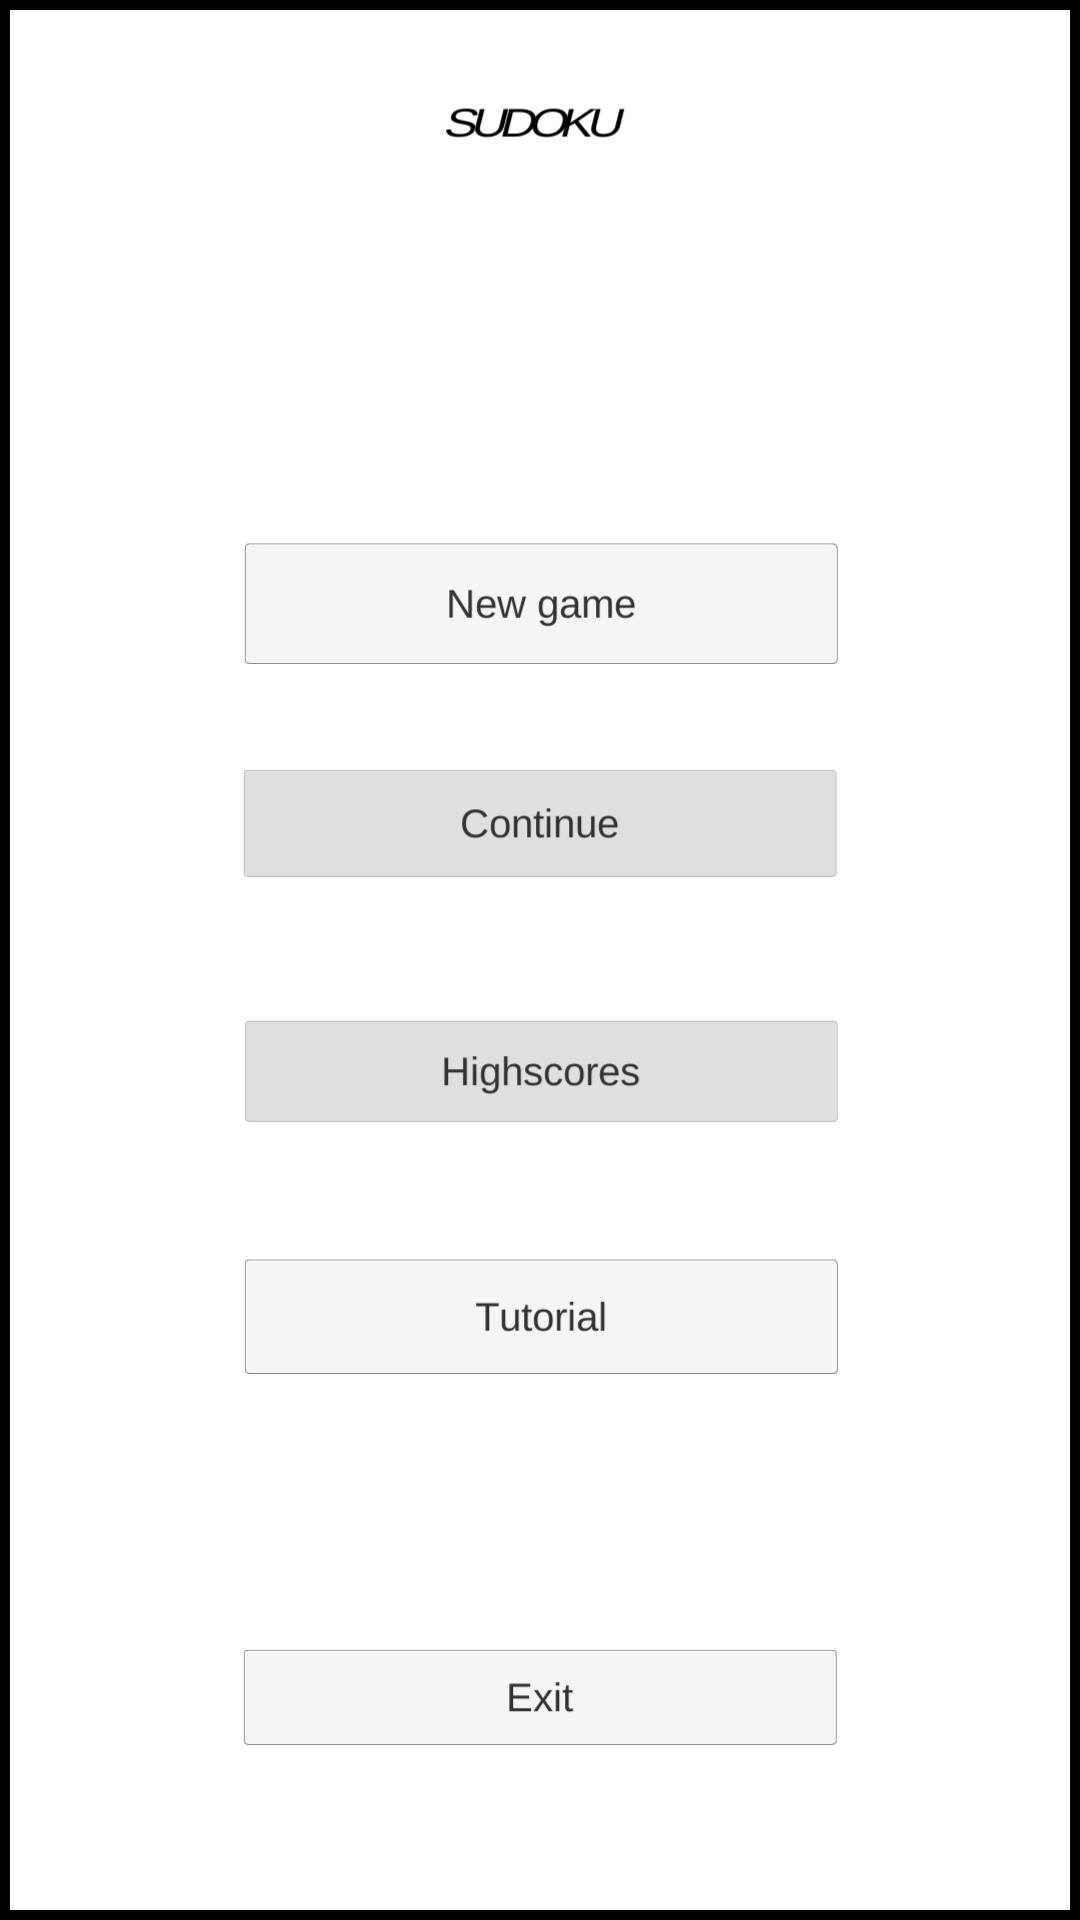
\includegraphics[width=5cm]{zrzuty/1.png}
	\caption{Menu główne}
	\label{fig:menu}
\end{figure}
Po wybraniu Highscores gracz otrzymuje listę najlepszych wyników podzielonych na poziomy trudności gry.
\begin{figure}[H]
	\centering
	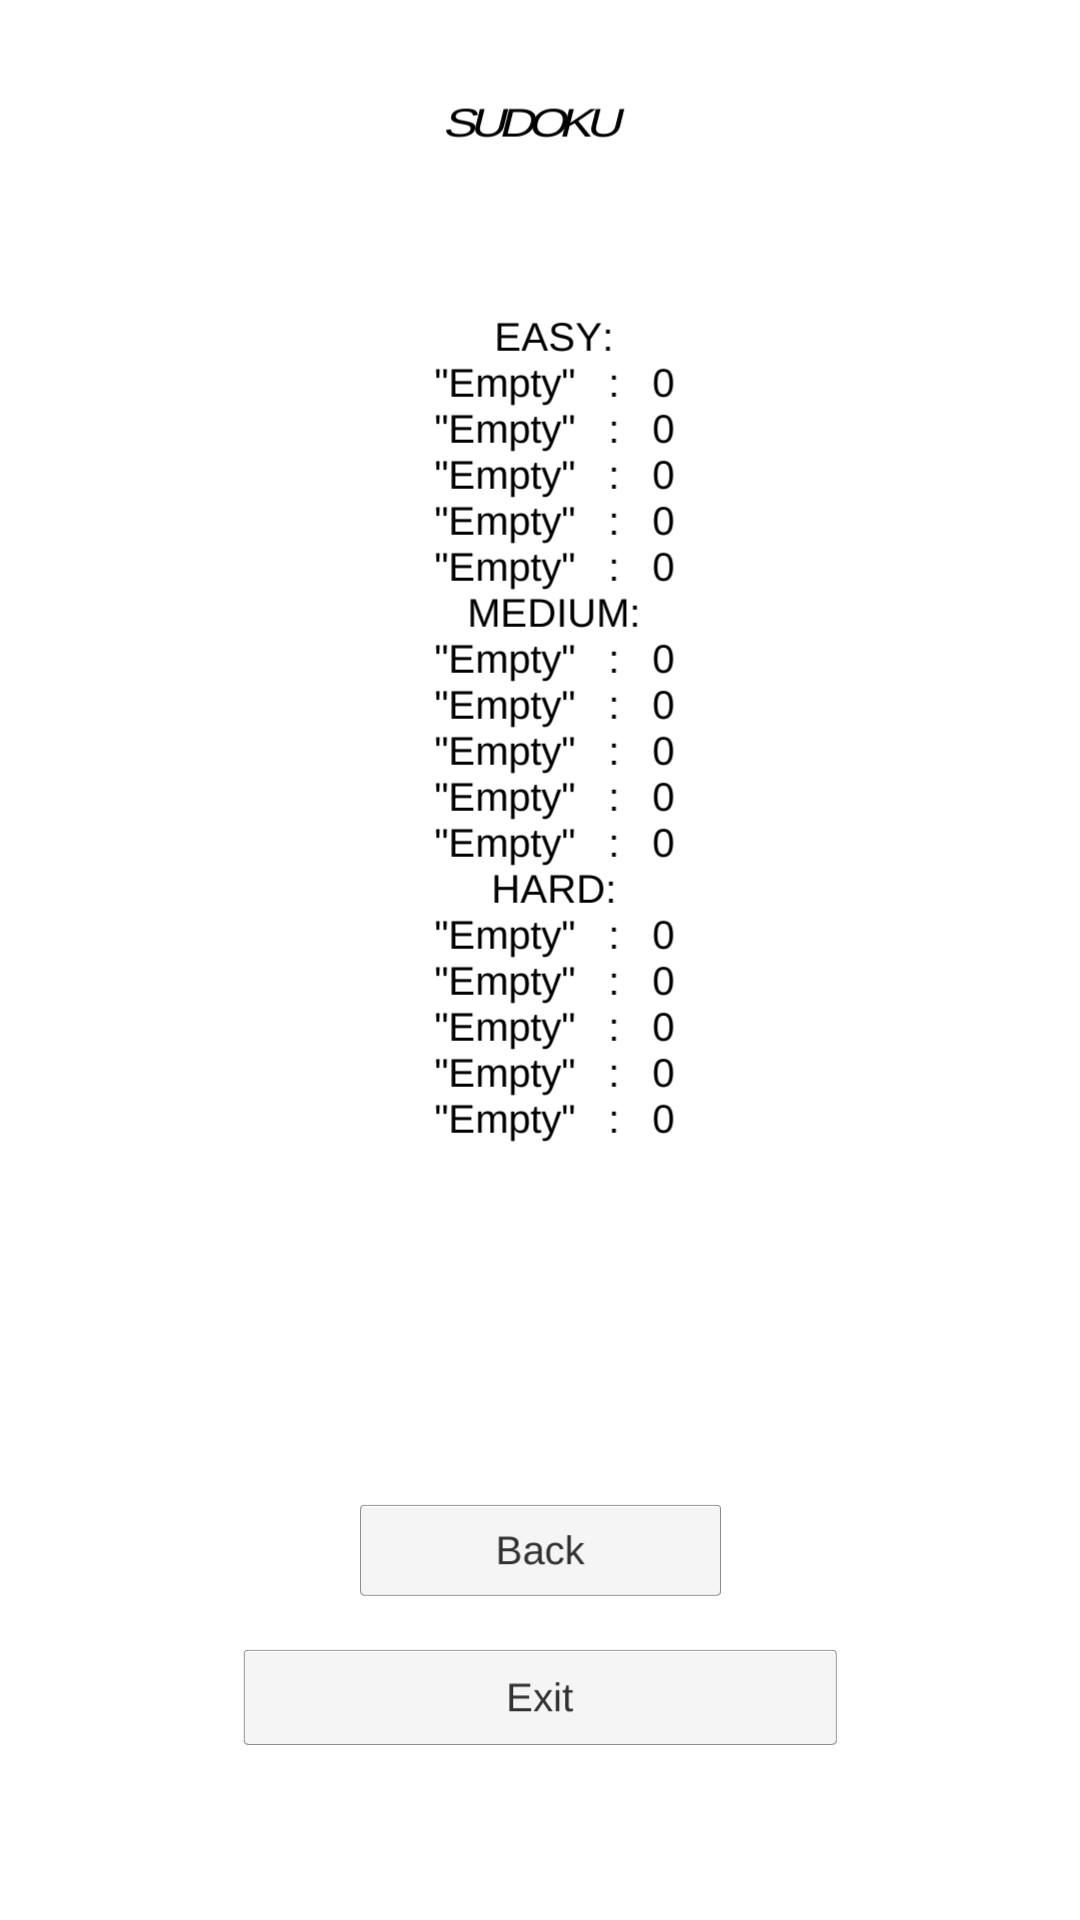
\includegraphics[width=5cm]{zrzuty/12.png}
	\caption{Lista najlepszych wyników}
	\label{fig:highscores}
\end{figure}
Po wyborze nowej gry gracz może podać swój nick poprzez wpisanie go w polu "Enter text...". Ma do wyboru trzy poziomy trudności: Easy, Medium oraz Hard.
\begin{figure}[H]
	\centering
	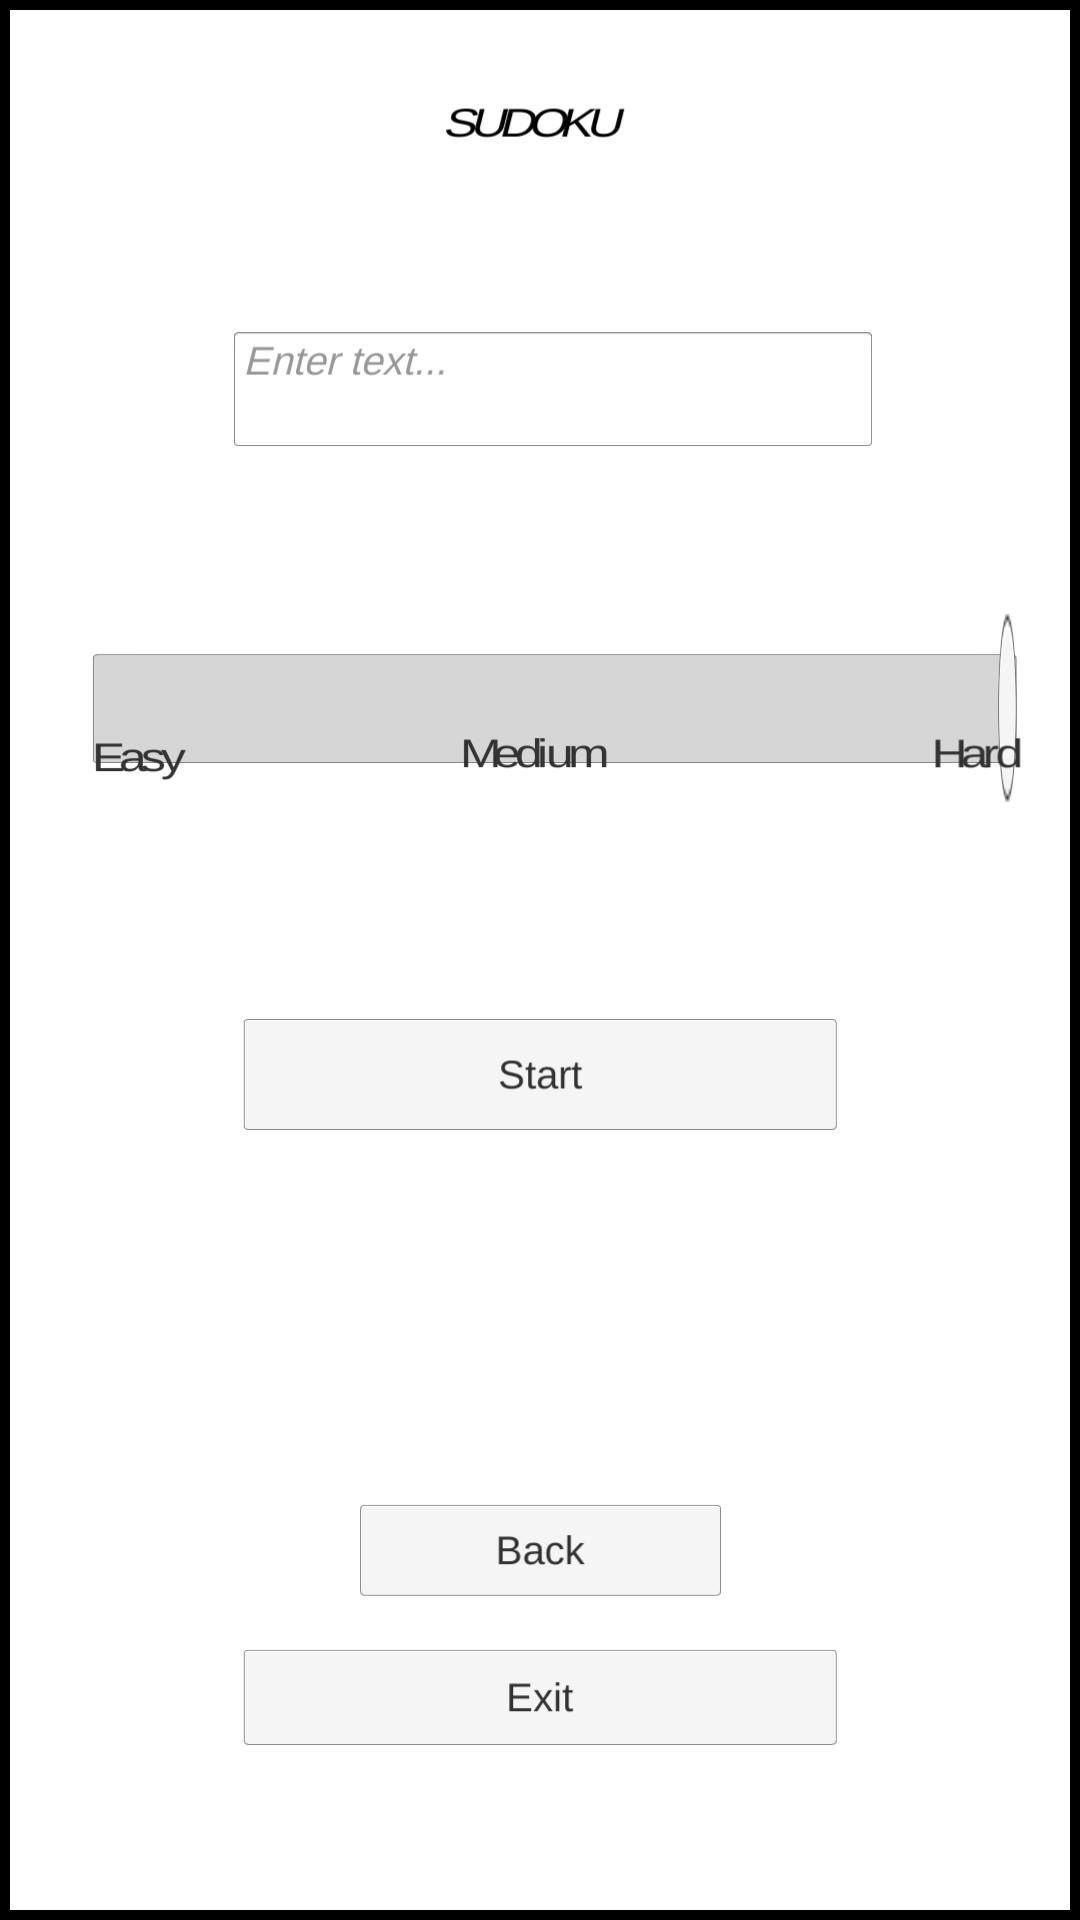
\includegraphics[width=5cm]{zrzuty/2.png}
	\caption{Menu nowej rozgrywki}
	\label{fig:menu2}
\end{figure} 
\begin{figure}[H]
	\centering
	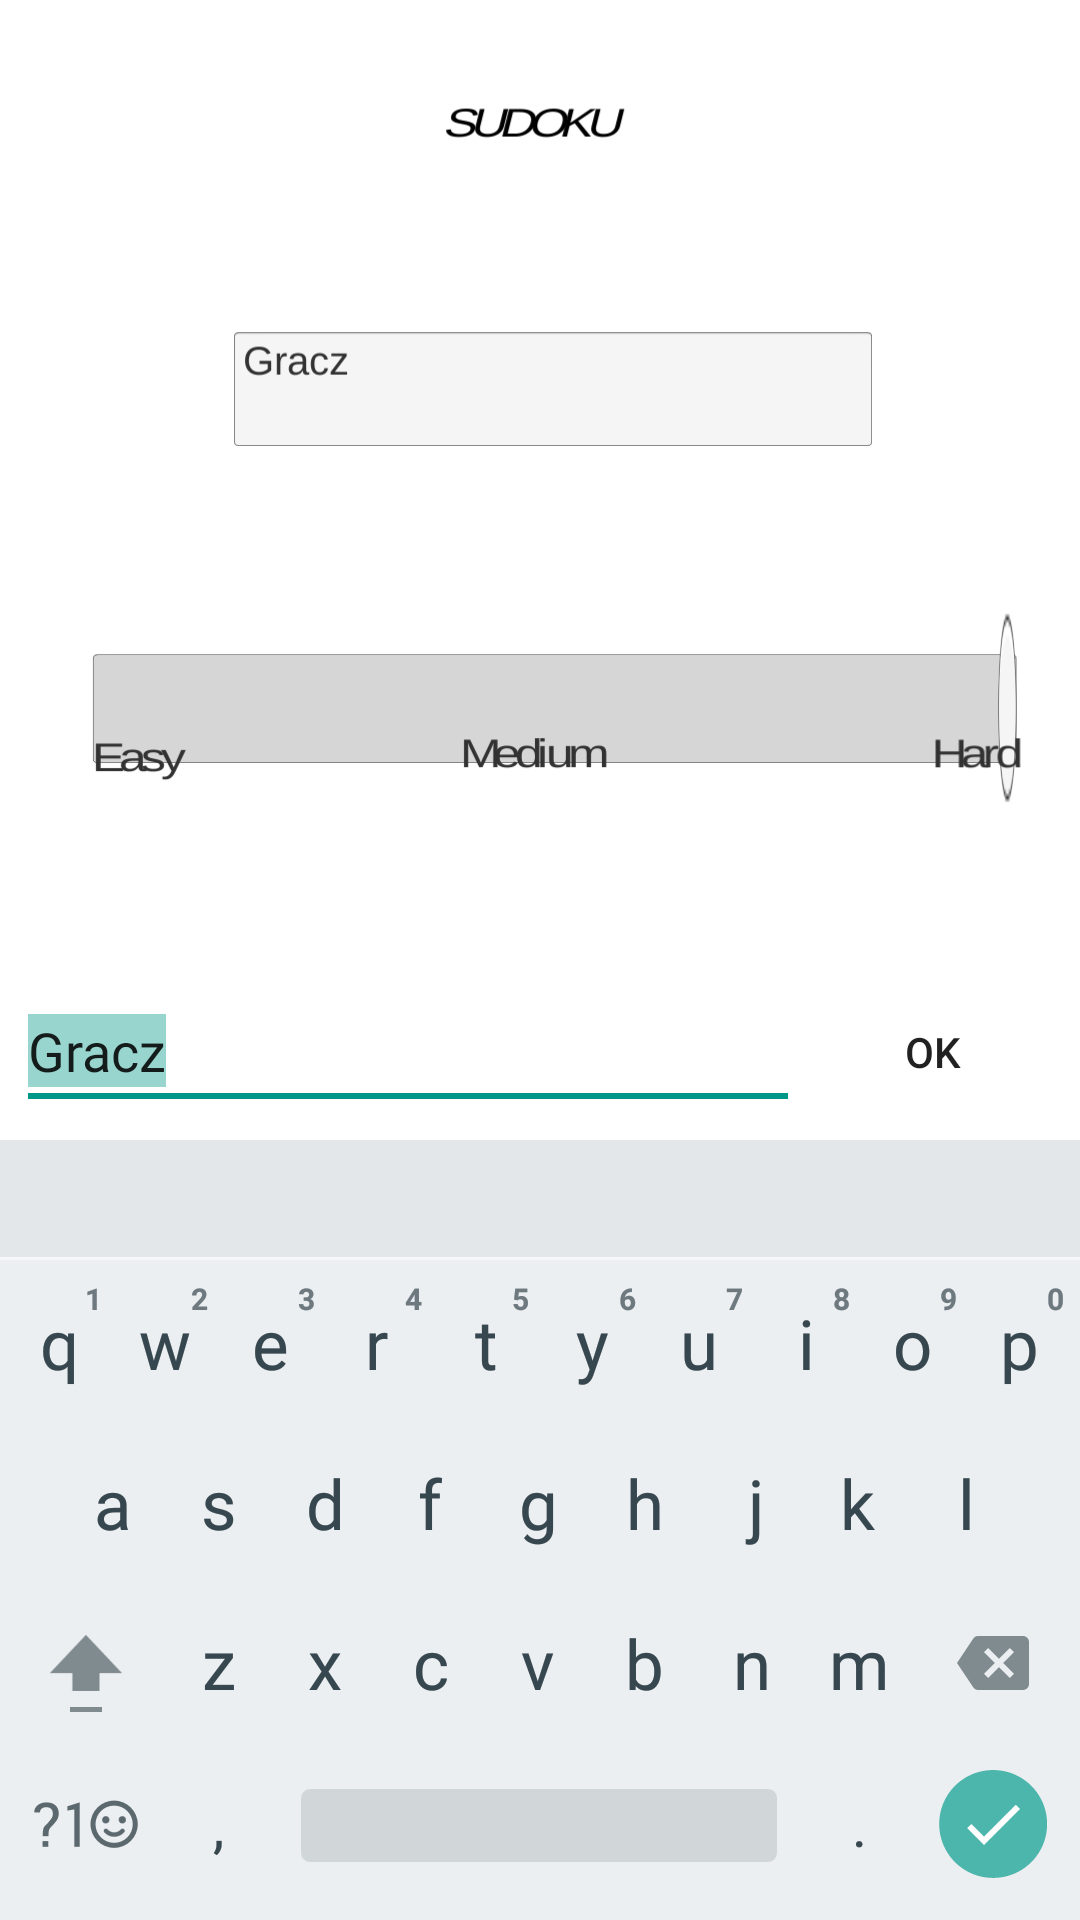
\includegraphics[width=5cm]{zrzuty/3.png}
	\caption{Wybór nicku}
	\label{fig:wybor_nicku}
\end{figure}
Po kliknięciu przycisku Start następuję wygenerowanie planszy i rozpoczyna się właściwa rozgrywka.  
\begin{figure}[H]
	\centering
	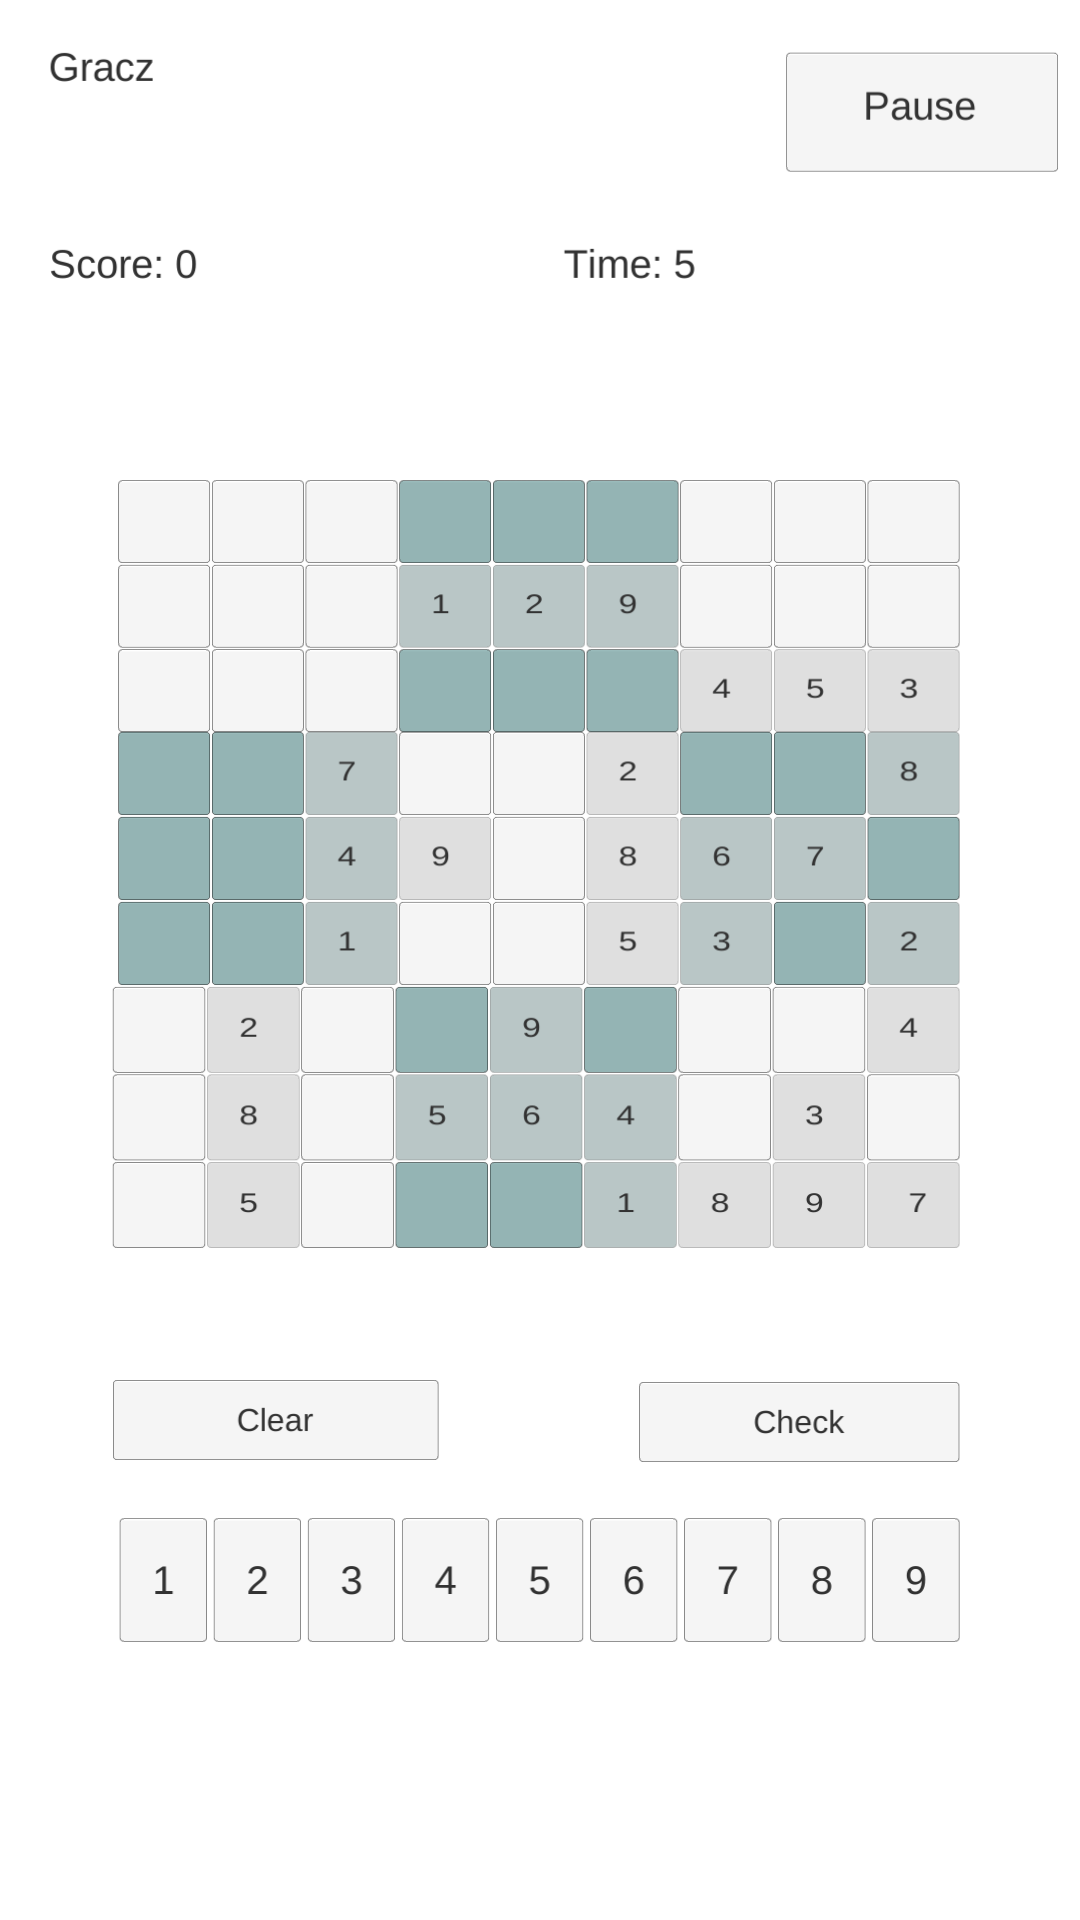
\includegraphics[width=5cm]{zrzuty/4.png}
	\caption{Nowa gra}
	\label{fig:nowagra}
\end{figure}
W trakcie gry mierzony jest czas oraz liczone są punkty. Po wyborze pustego pola zaznaczane jest ono na czerwono i gracz poprzez wybór cyfry z dolnego paska wprowadza wartość do pola.
\begin{figure}[H]
	\centering
	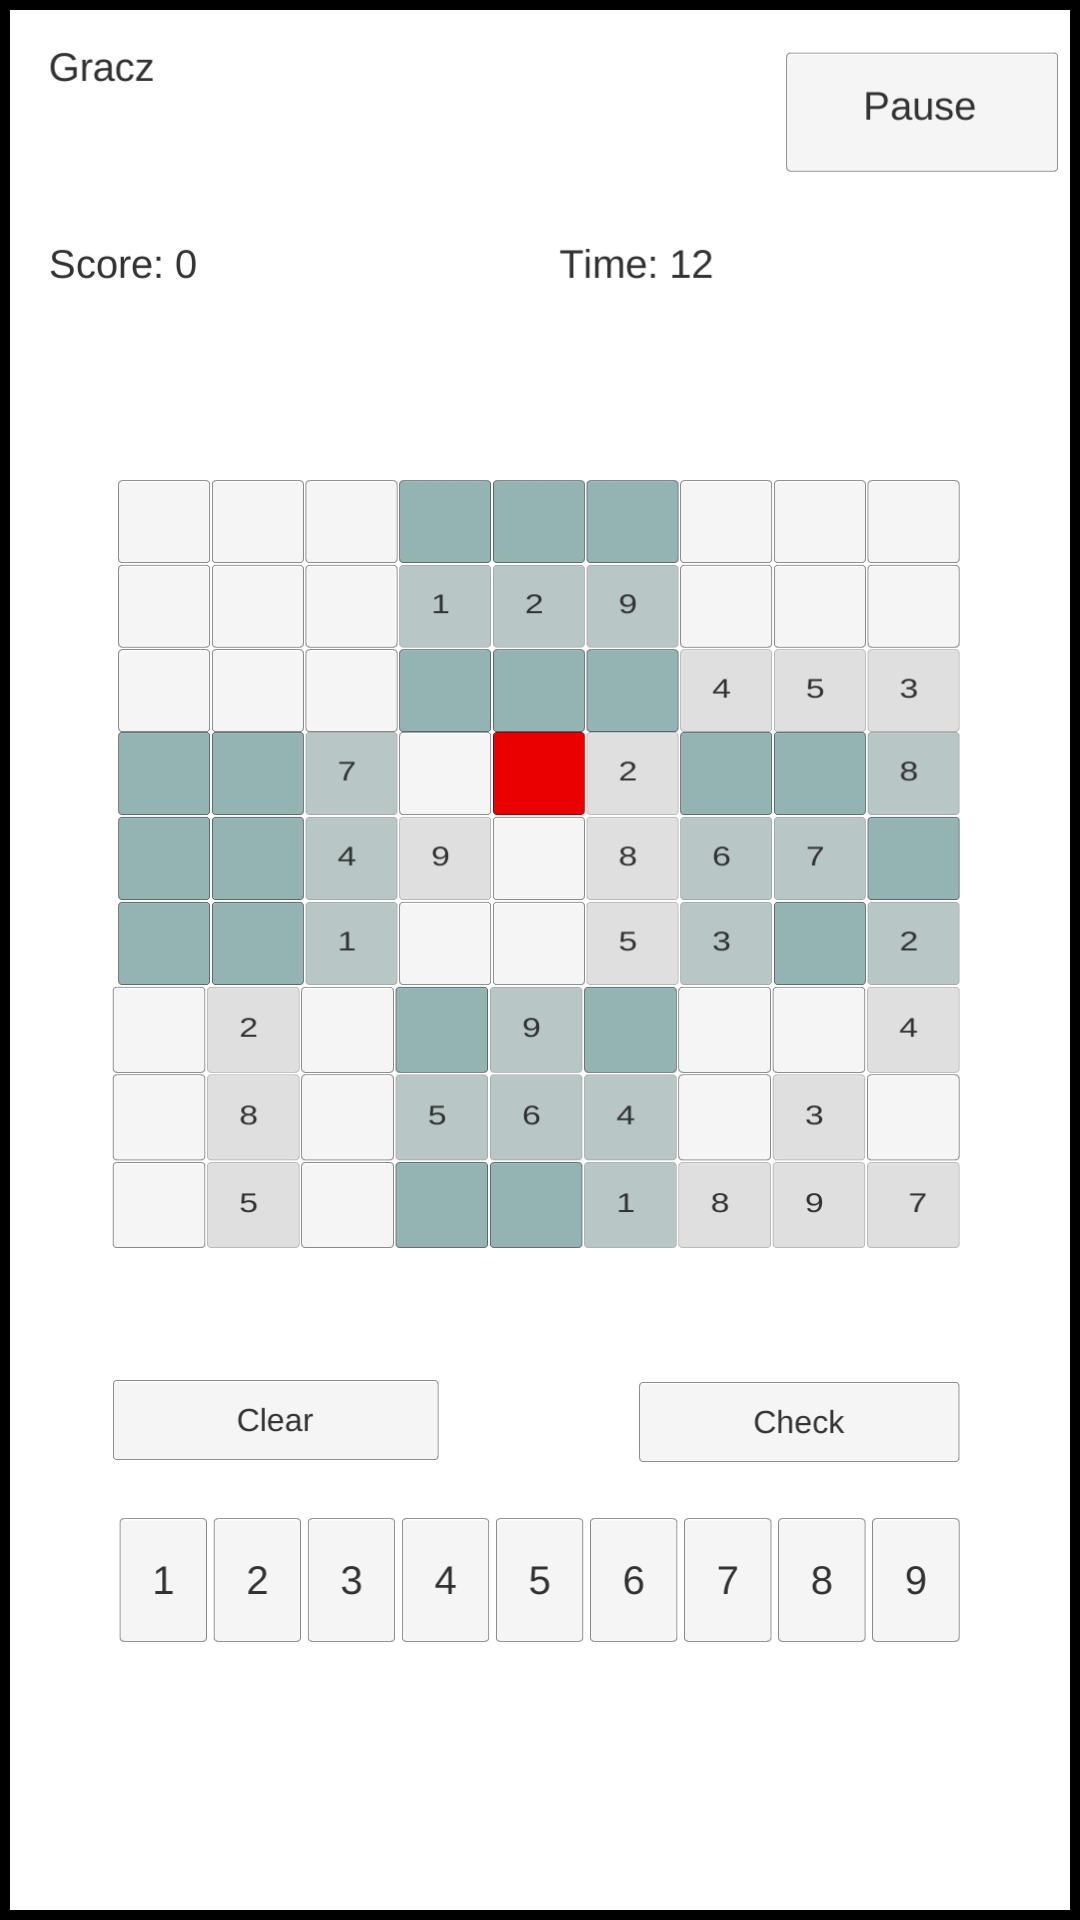
\includegraphics[width=5cm]{zrzuty/5.png}
	\caption{Wybór pola}
	\label{fig:wybor_pola}
\end{figure}
\begin{figure}[H]
	\centering
	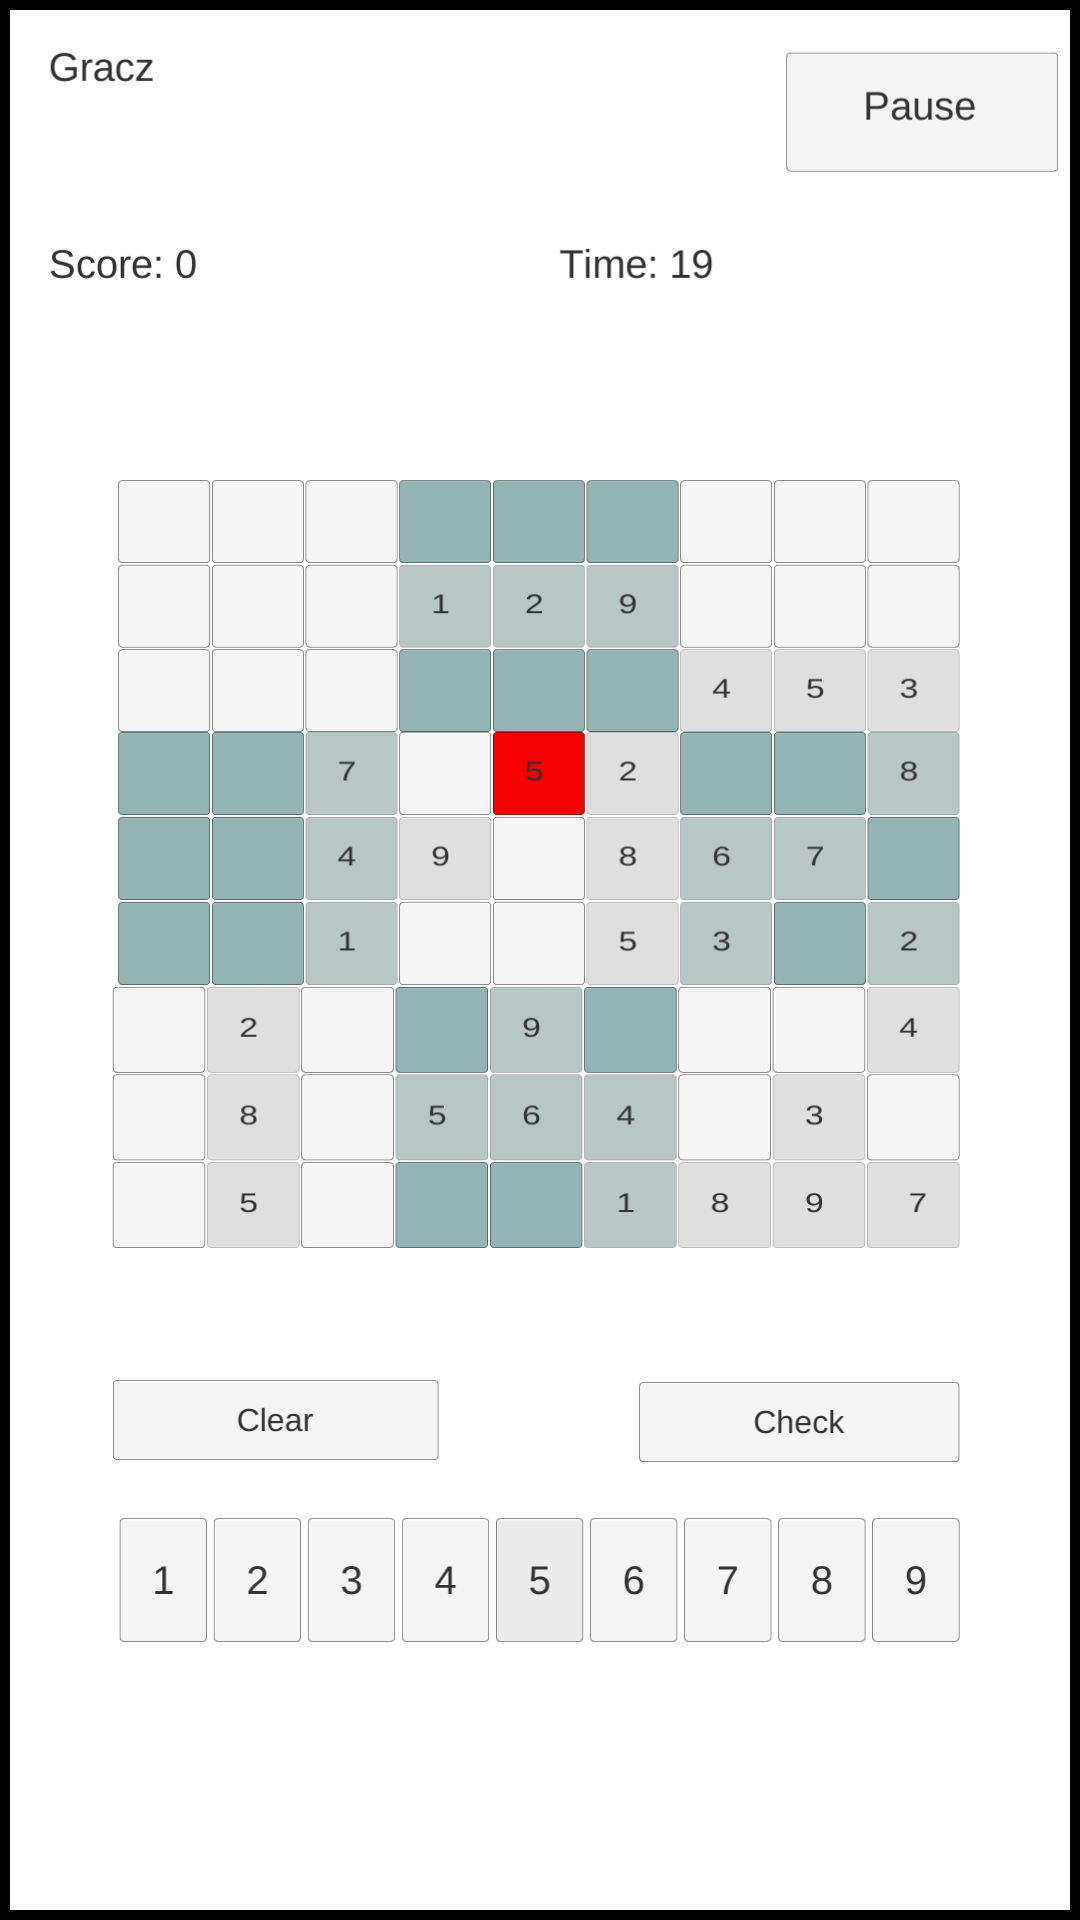
\includegraphics[width=5cm]{zrzuty/6.png}
	\caption{Wprowadzenie wartości}
	\label{fig:wprowadzenie_wartosci}
\end{figure}
Gracz ma możliwość sprawdzenia zgodności wprowadzonych wartości z zasadami Sudoku poprzez kliknięcie przycisku Check. W przypadku złamania zasad pojawia się napis "You have errors".
\begin{figure}[H]
	\centering
	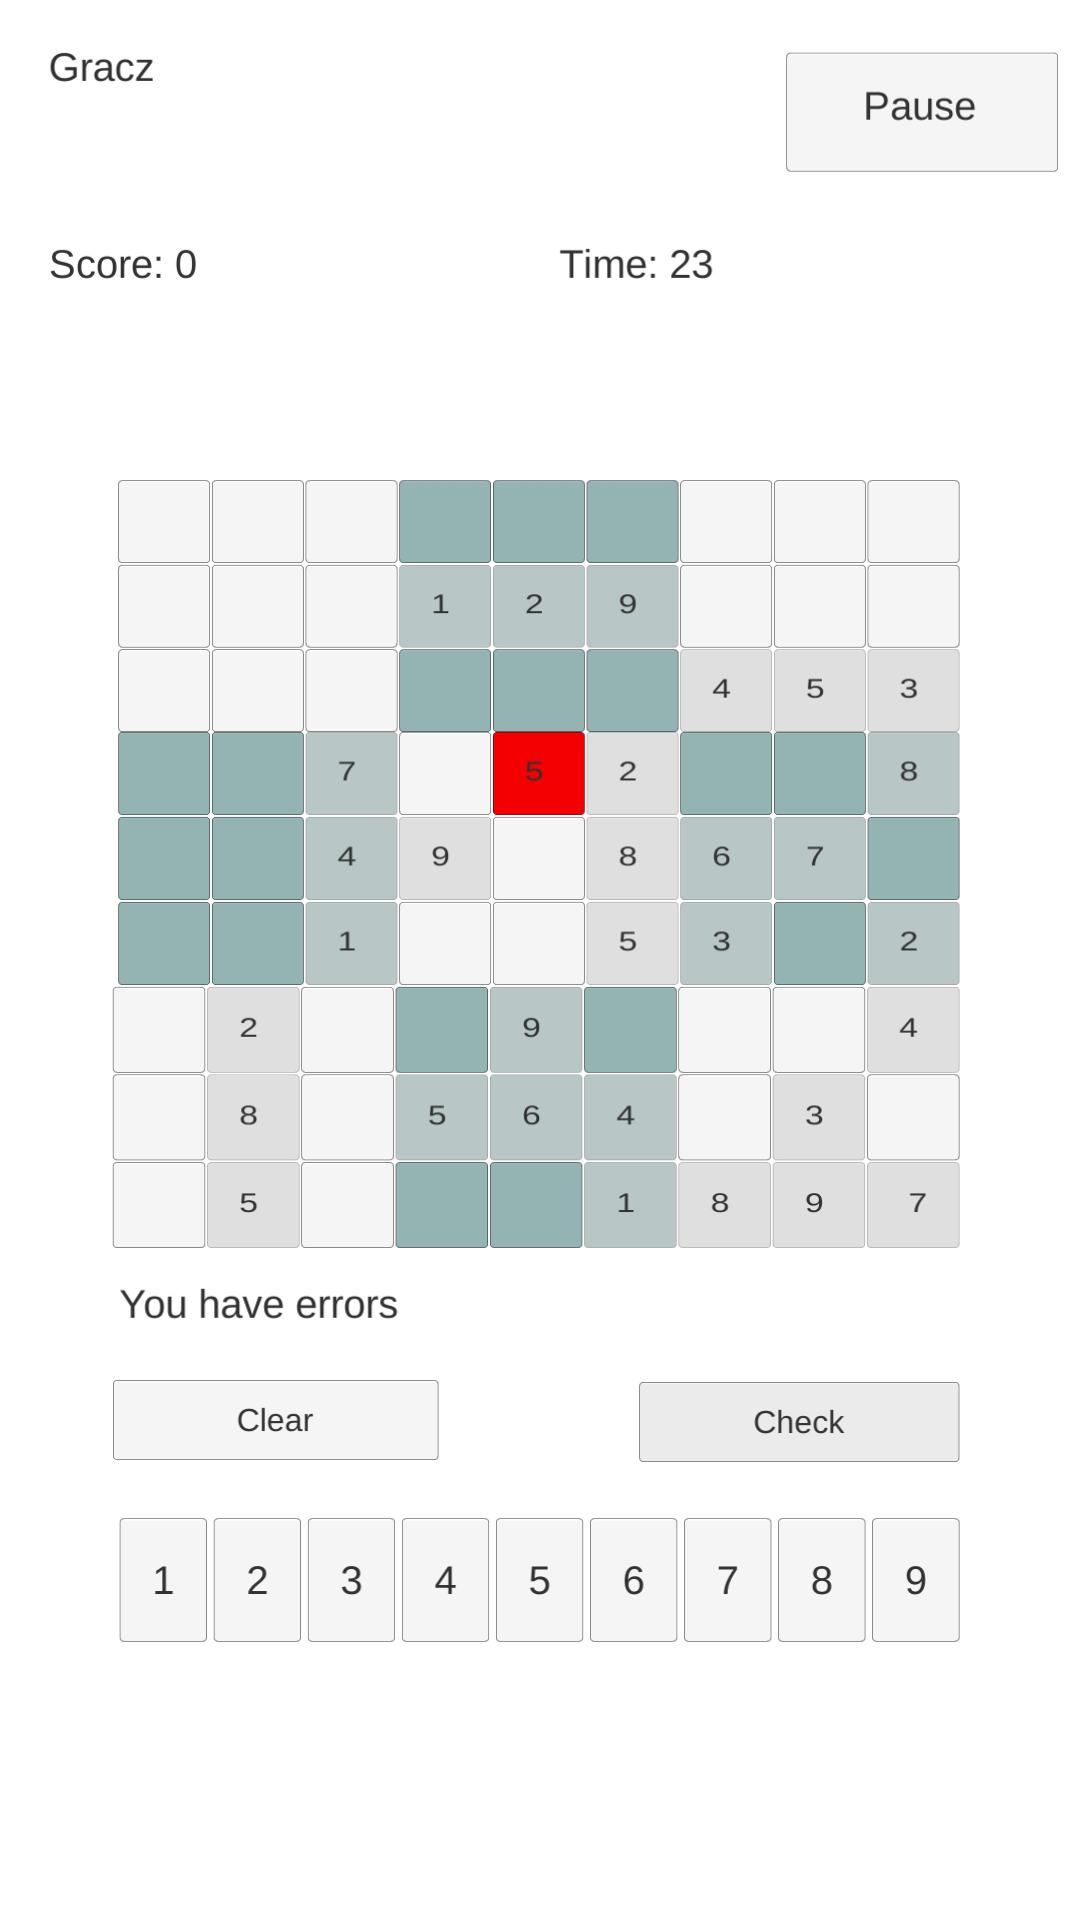
\includegraphics[width=5cm]{zrzuty/7.png}
	\caption{Sprawdzenie planszy w sytuacji złamania zasad Sudoku}
	\label{fig:check_errors}
\end{figure}
Gracz może wyczyścić pole przyciskiem Clear. Wiąże się to jednak z otrzymaniem ujemnych punktów.
\begin{figure}[H]
	\centering
	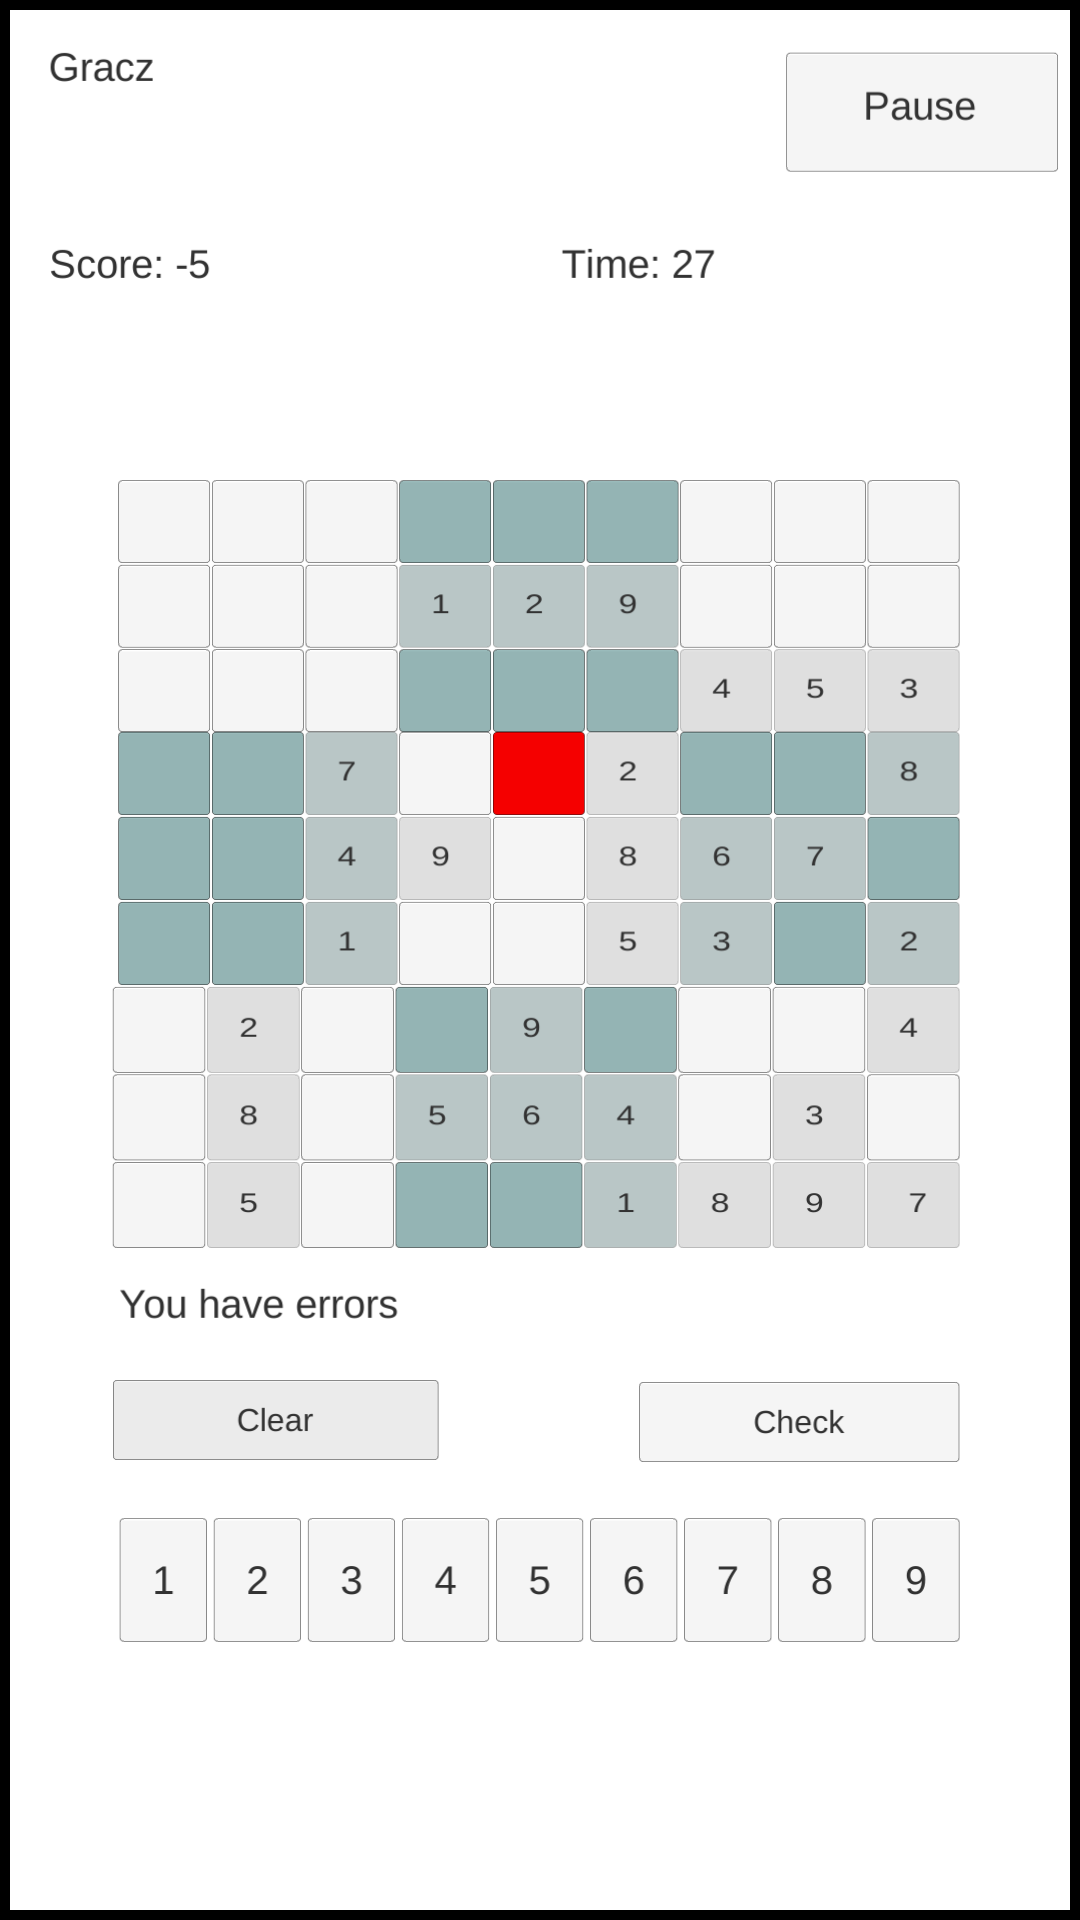
\includegraphics[width=5cm]{zrzuty/8.png}
	\caption{Wyczyszczenie pola}
	\label{fig:clear}
\end{figure}
W przypadku sprawdzenia planszy i braku niezgodności wyświetlany jest komunikat "You don't have errors".
\begin{figure}[H]
	\centering
	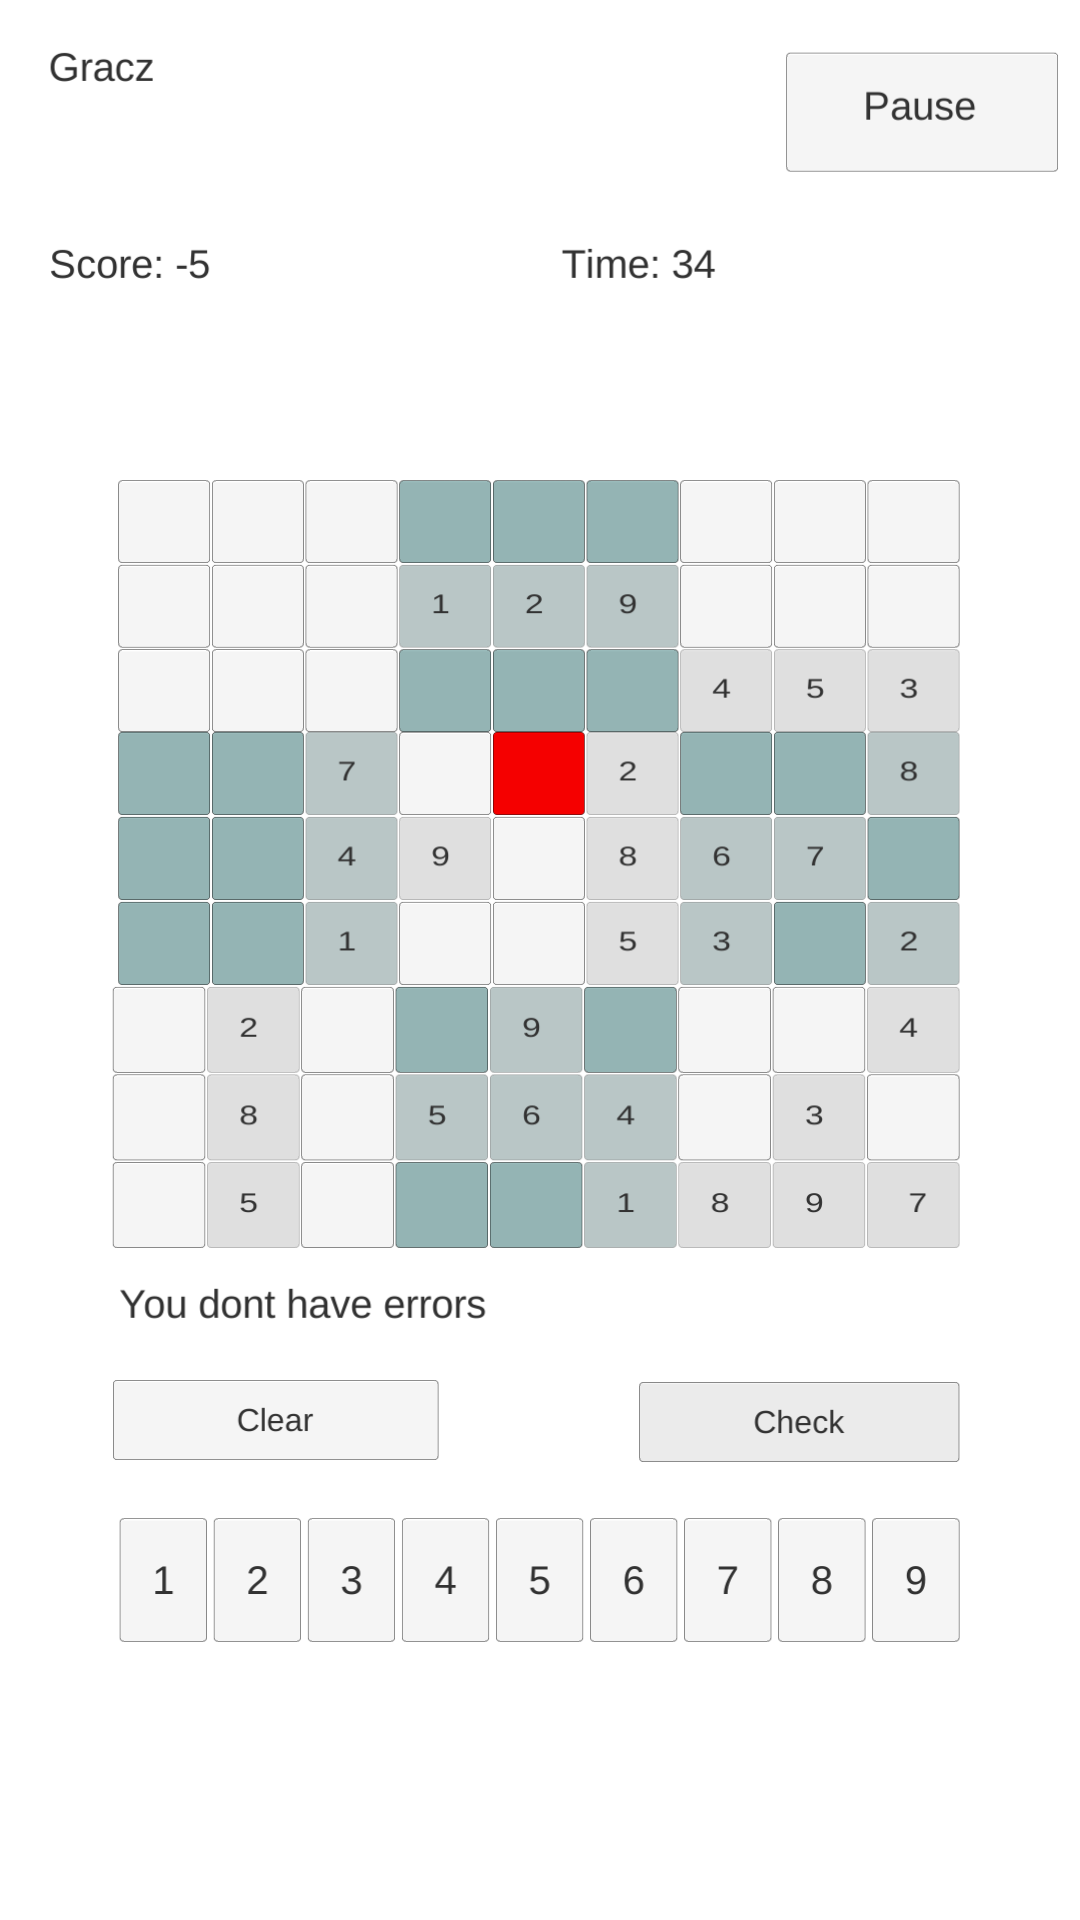
\includegraphics[width=5cm]{zrzuty/9.png}
	\caption{Sprawdzenie planszy w przypadku braku niezgodności}
	\label{fig:check_ok}
\end{figure}
Po kliknięciu przycisku Pause następuje wstrzymanie rozgrywki i pojawia się lista opcji opcji do wyboru. Gracz może wrócić do gry, włączyć/wyłączyć muzykę, wyjść do menu głównego lub wyłączyć grę.
\begin{figure}[H]
	\centering
	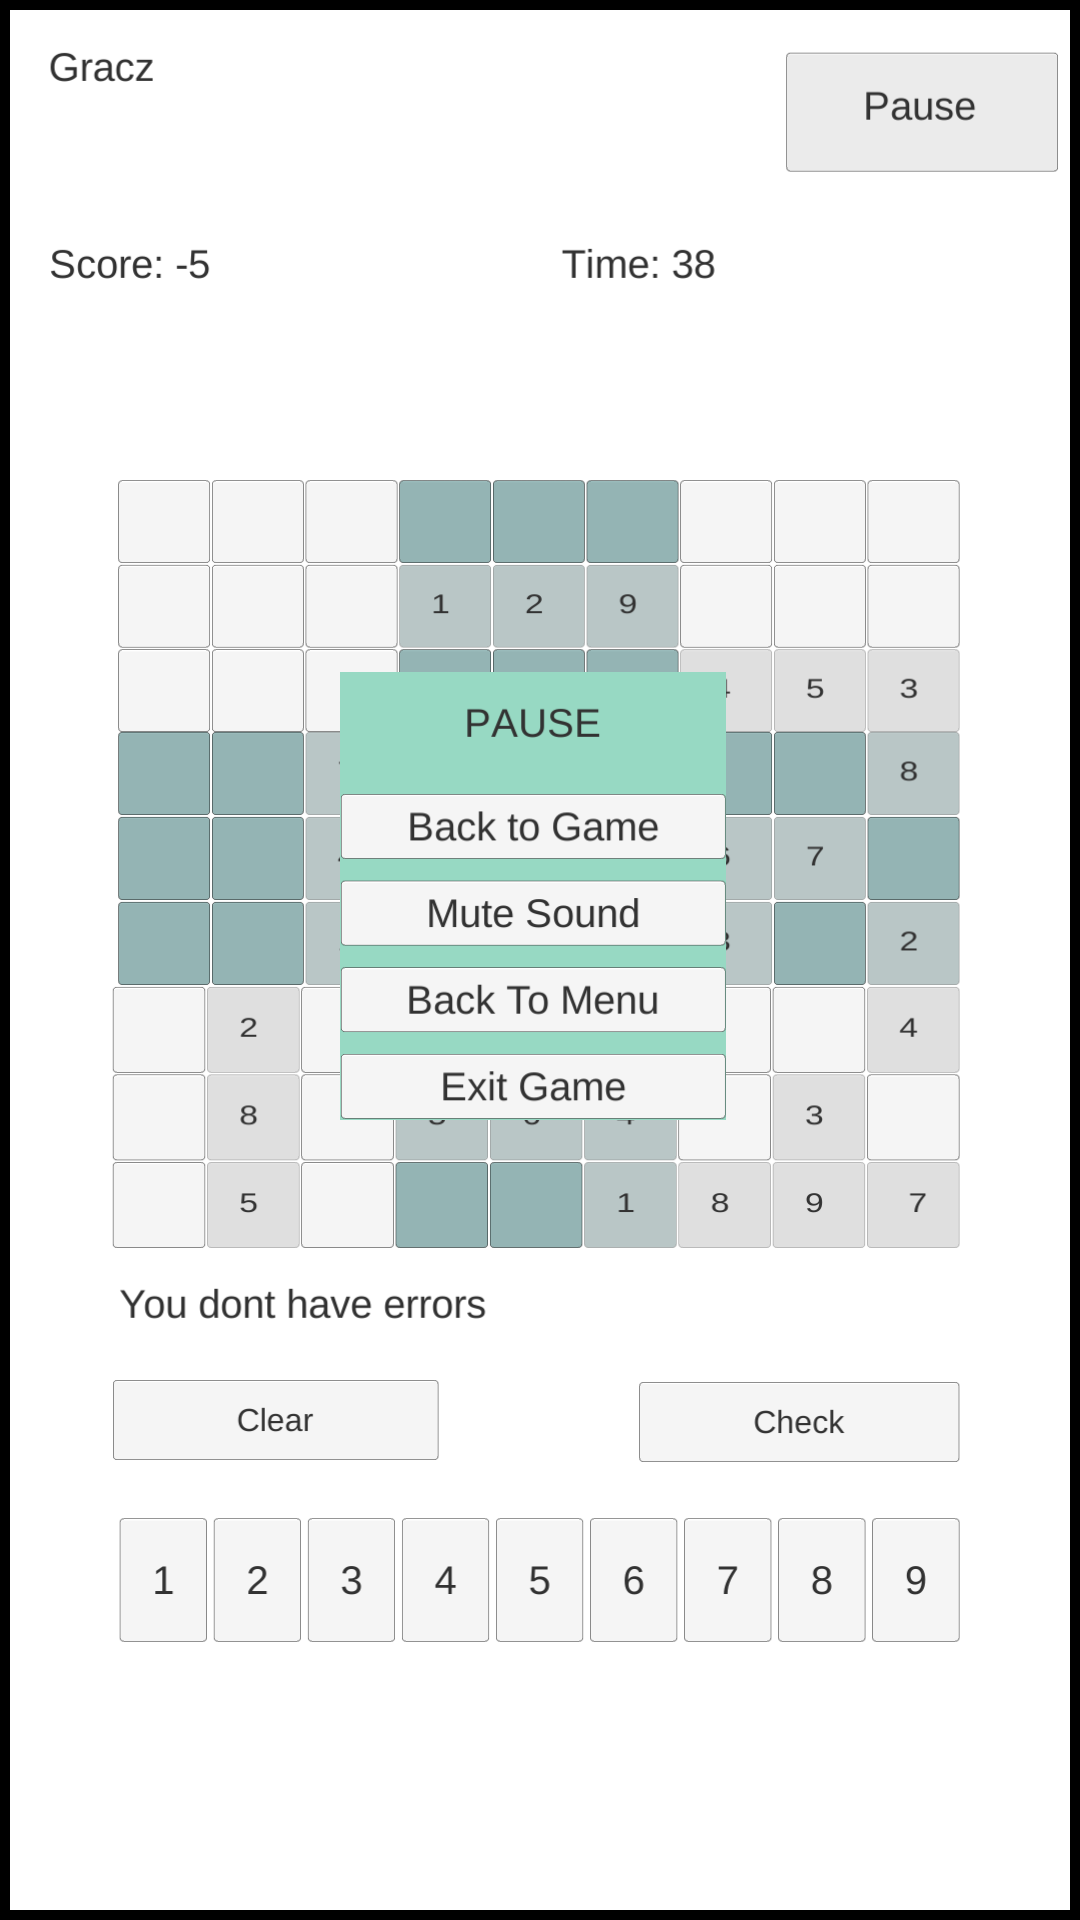
\includegraphics[width=5cm]{zrzuty/10.png}
	\caption{Menu w trakcie gry przy włączonej muzyce}
	\label{fig:menu_pause}
\end{figure}
\begin{figure}[H]
	\centering
	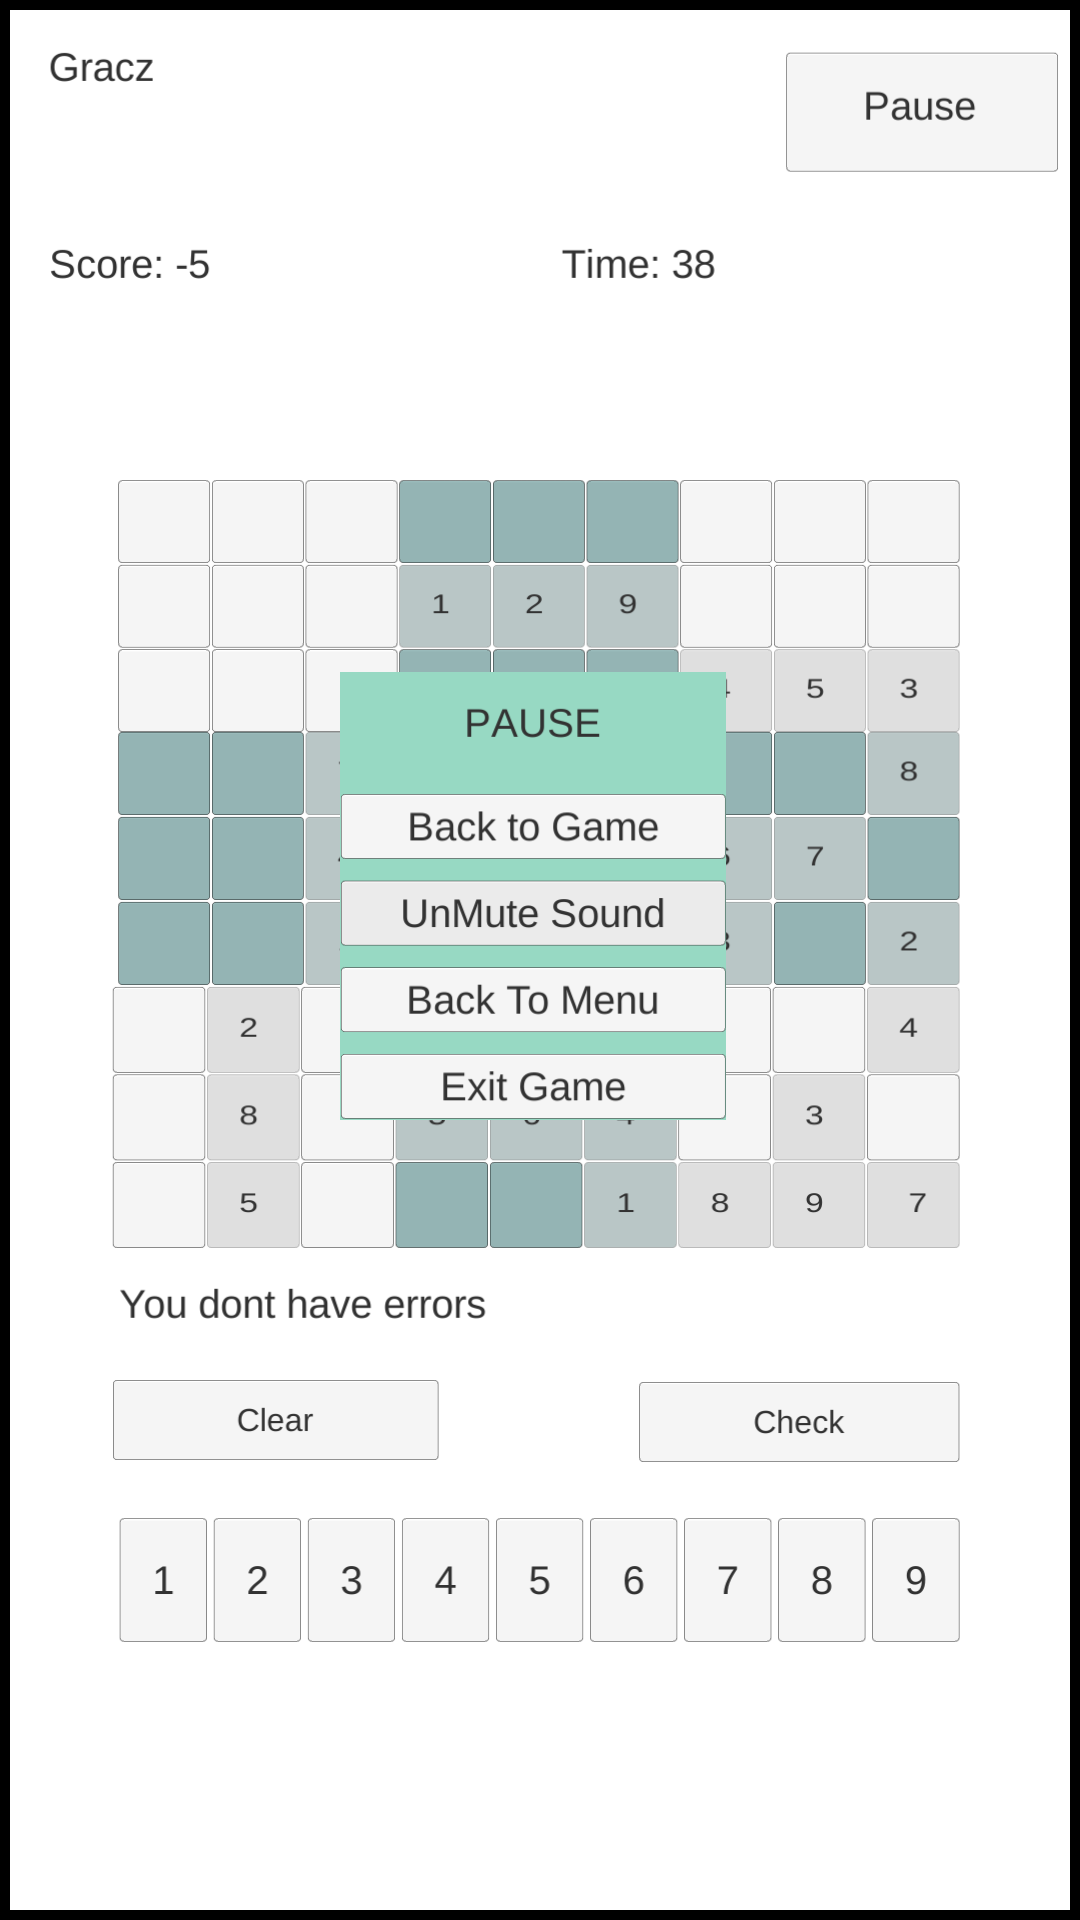
\includegraphics[width=5cm]{zrzuty/11.png}
	\caption{Menu w trakcie gry przy wyłączonej muzyce}
	\label{fig:menu_pause2}
\end{figure}





\vfill
	\newpage
\section{Struktura aplikacji}
\subsection{Moduły}
W aplikacji można wyodrębnić następujące moduły:
\begin{itemize}
	\item GUI
	\item Logic
	\item SoundControl
	\item Utilities
	\item Plugins
\end{itemize}
\begin{figure}[H]
	\centering
	\includegraphics[width=8cm]{diagramy/moduly.png}
	\caption{Moduły programu}
	\label{fig:modules}
\end{figure}

Moduł Logic jest odpowiedzialny za mechanikę gry. Zapewnia on zachowanie zasad gry w sudoku. Generuje plansze według podanego poziomu trudności. Ponadto odpowiada za dodatkową funkcjonalność. Dodatkowe udostępnione opcje to: 
-możliwość cofania ruchu gracz( działa to na zasadzie przywrócenia poprzedniego stanu planszy, stanu te przechowujemy w liście dzięki czemu możemy przejść od ostatniego ruchu do pierwszego, a nawet zresetować planszę do stanu pierwotnego), 
-wyświetlanie cyfr możliwych do wstawienia( jest to realizowane poprzez ustawienie przycisków wyboru cyfry na aktywne, zaś tych przycisków, które nie spełniają zasad na nieaktywne),
- kontynuowanie niedokończonej rozgrywki( jest możliwe dzięki zapisywaniu stanu planszy w pamięci telefonu, a także nicku gracza i jego wyniku),
- tablica wyników, która przechowuje wyniki odpowiednio dla poziomu łatwego, normalnego oraz trudnego w dwóch kategoriach odpowiadających trybom gry(klasyczny, gra na czas) w których zostały zdobyte. 


Moduł SoundControl służy do kontrolowania muzyki grającej w tle, a także różnorakich efektów dźwiękowych m.in. dźwięk wygranej, dźwięk naciskania przycisków, melodia pobicia rekordu.


Moduł GUI jest odpowiedzialny za odpowiednie rozlokowanie elementów menu i widoku gry. Ponadto pośredniczy on między akcjami gracza, a modułem logiki. Wszelkie interakcja z aplikacją odbywa się poprzez tą warstwę i jej elementy(przyciski).


Moduł Utilities przechowuje pomniejsze pomocne klasy.

Moduł Plugins zawiera klasę do obsługi JSON.
\subsection{Diagramy klas}

\begin{figure}[H]
	\centering
	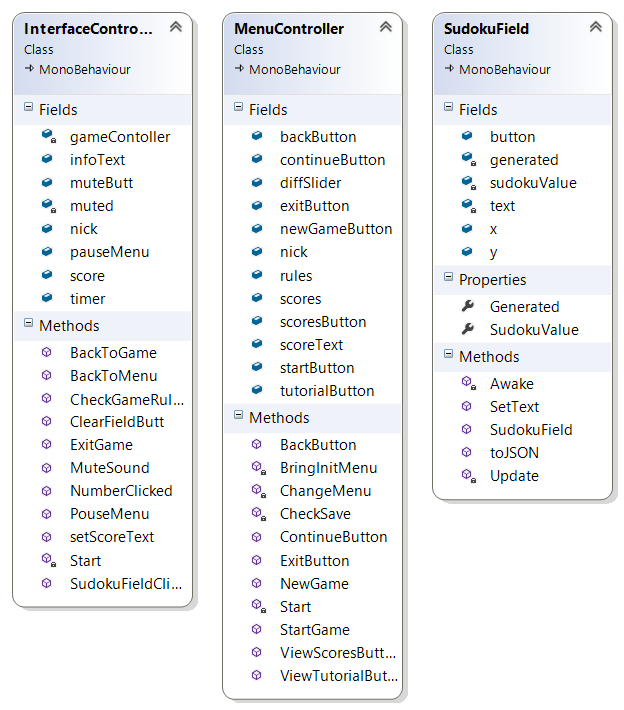
\includegraphics[width=5cm]{diagramy/class_gui.png}
	\caption{Diagram klas dla modułu GUI}
	\label{fig:class_gui}
\end{figure}
\begin{figure}[H]
	\centering
	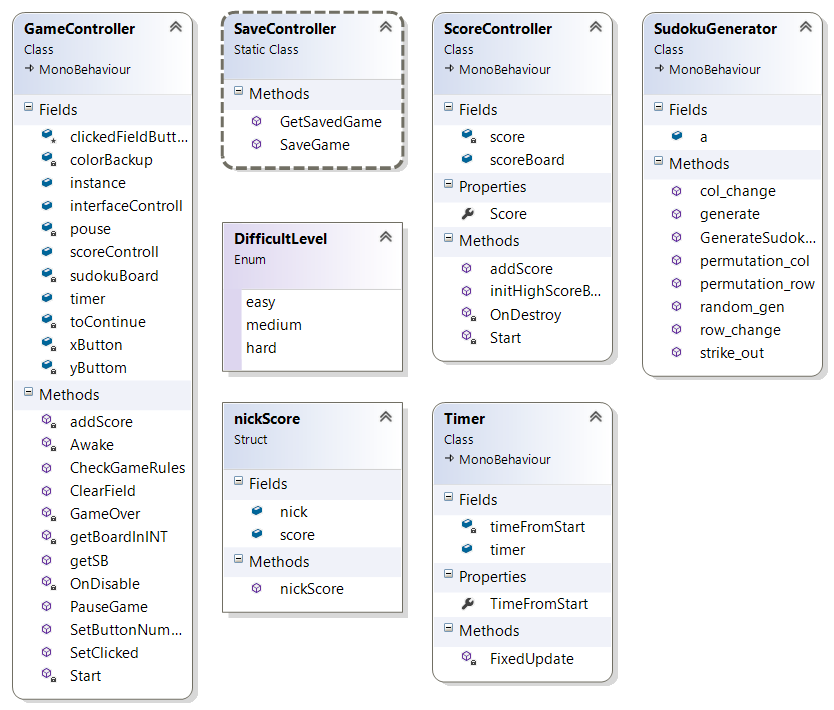
\includegraphics[width=5cm]{diagramy/class_logic.png}
	\caption{Diagram klas dla modułu Logic}
	\label{fig:class_logic}
\end{figure}
\begin{figure}[H]
	\centering
	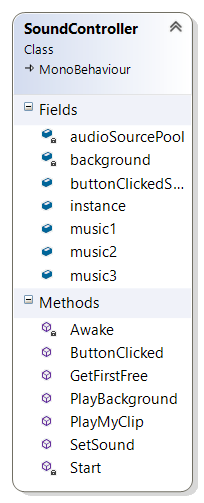
\includegraphics[width=5cm]{diagramy/class_sound.png}
	\caption{Diagram klas dla modułu Sound}
	\label{fig:class_sound}
\end{figure}
\begin{figure}[H]
	\centering
	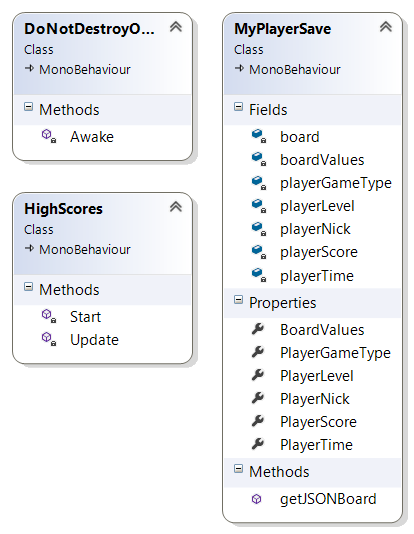
\includegraphics[width=5cm]{diagramy/class_util.png}
	\caption{Diagramy klas dla modułu Utilities}
	\label{fig:class_util}
\end{figure}
\newpage
\subsection{Algorytm generowania plansz}
W pierwszym kroku generowana jest plansza spełniająca zasady Sudoku, to znaczy:
\begin{itemize}
	\item Każda cyfra może się pojawić tylko raz w każdym wierszu,
	\item Każda cyfra może się pojawić tylko raz w każdej kolumnie,
	\item Każda cyfra może się pojawić tylko raz w każdym obszarze.
\end{itemize}
Przyjmuje ona następującą postać
\begin{figure}[H]
	\centering
	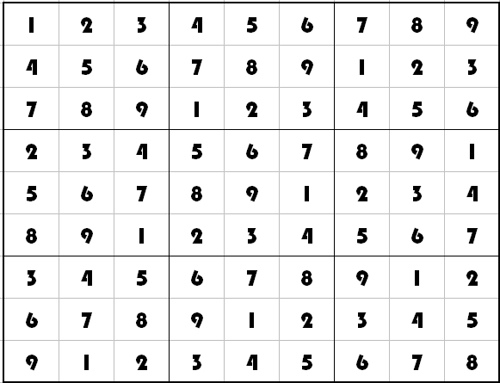
\includegraphics[width=8cm]{zrzuty/plansza.png}
	\caption{Plansza po pierwszym wygenerowaniu}
	\label{fig:first_gen_board}
\end{figure}
Następnie, aby uzyskać różne warianty planszy dokonuje się szeregu transformacji, które nie będą prowadzić do złamania zasad gry. Wśród nich mamy:
\begin{itemize}
	\item zamiana dwóch wierszy w ramach tej samej grupy
	\begin{figure}[H]
		\centering
		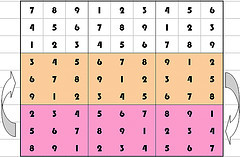
\includegraphics[width=8cm]{zrzuty/shuffle.png}
		\caption{Zamiana wierszy}
		\label{fig:szuffle1}
	\end{figure}
	\item zamiana dwóch kolumn w ramach tej samej grupy
	\item zamiana dwóch grup wierszy (9x3)
	\begin{figure}[H]
		\centering
		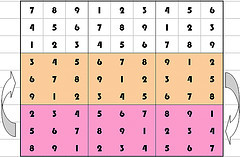
\includegraphics[width=8cm]{zrzuty/szufflee.png}
		\caption{Zamiana grup wierszy}
		\label{fig:szuffle2}
	\end{figure}
	\item zamiana dwóch grupy kolumn
\end{itemize}
Kolejnym krokiem jest wyczyszczenie części pól. Czyszczone są pola, które nie zakłócają warunku jednego możliwego poprawnego rozwiązania.
\vfill
\newpage
\section{Testy i wdrożenia}
\subsection{Wdrożenie}
Aplikacja została zaprojektowana i zrealizowana w celach niekomercyjnych, dlatego nie została opublikowana w Sklepie Play. Jednakże udostępniliśmy cały projekt poprzez publiczne repozytorium github z licencją opensource MIT.
\subsection{Testy}
Aplikacja została przetestowana na poniższych modelach telefonów:
\begin{itemize}
\item LG Spirit - Android 6.0 - Gra działała płynnie, nie wykryto błędów uniemożliwiających zakończenie gry,
\item Xiaomi Mi4c - 5.1.1 - jak wyżej.	
\end{itemize}

\subsection{Wnioski}
Na podstawie testów i komentarzy osób testujących oraz spełnionych wymagań, projekt można uznać za pomyślnie zakończony.


\vfill
\newpage
\section{Rozwój}
Projekt w przyszłości można rozwinąć o kilka rzeczy:
\begin{itemize}
\item połączenie z mediami społecznościowymi, t.j. facebook, twitter,
\item tabele wyników przechowywaną globalnie na serwerze,
\item system wyświetlający reklamy,
\item system rejestracji użytkowników, dla zapewnienia unikalnych nicków graczy.
\end{itemize}

	
	% latex(szybka kompilacja),bibtex,kompilacja,kompilacja
%\bibliographystyle{plain}% plain/abbrv/alpha
%\bibliography{bibliografia}%plik .bib
\end{document}


